Часто в супутникових даних зустрічаються ситуації, коли в датасеті є неповні знімки
(рис. \ref{fig:non-full}).

\begin{figure}[H]
	\centering
	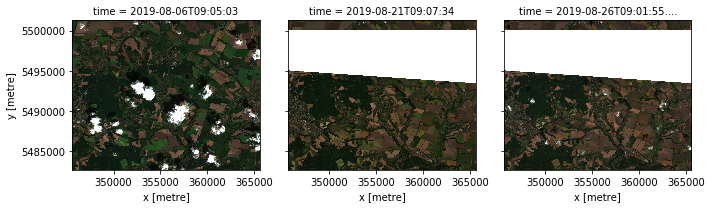
\includegraphics[width=0.7\textwidth]{images/image14}
	\caption{Приклад неповних даних}
	\label{fig:non-full}
\end{figure}

На жаль, саме через такі випадки в безхмарному результуючому знімку можна
помітити, що на деяких частинах зображення (рис. \ref{fig:cloudless-result})
можна побачити різницю між колірними просторами, а саме: на одному з регіонів може
бути більше зелені або, навпаки, менше, що буде одразу помітно на цілому
зображенні.

Тому постає задача розв'язання цієї проблеми. Необхідно розглянути алгоритми,
мета яких --- переведення колірного простору між зображеннями.

\begin{figure}[H]
	\centering
	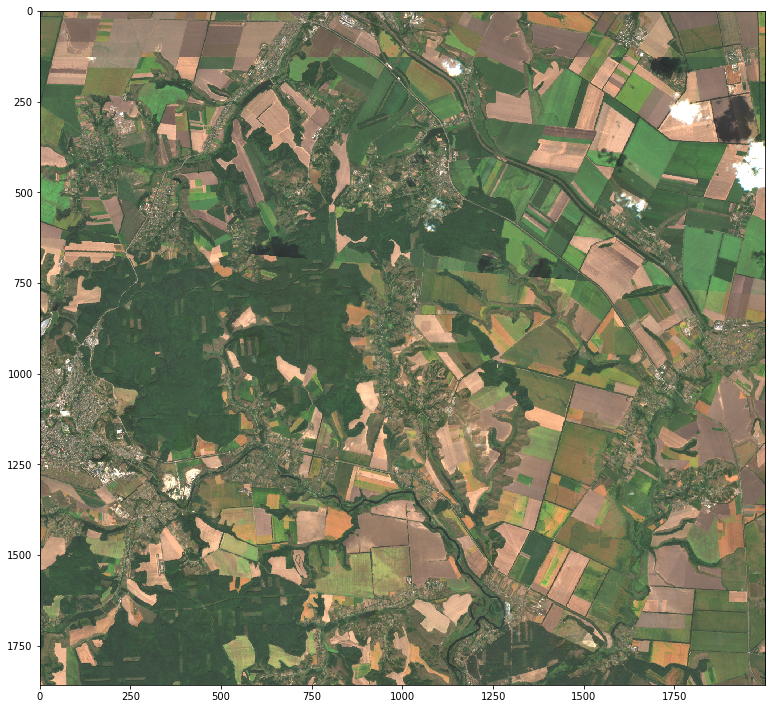
\includegraphics[width=0.5\textwidth]{images/image15}
	\caption{Результат обробки алгоритмом безхмарного композитування з дефектами склейки
	\label{fig:cloudless-result} }
\end{figure}
